\section{Solarzelle}

\subsection{Aufbau Solarzelle}
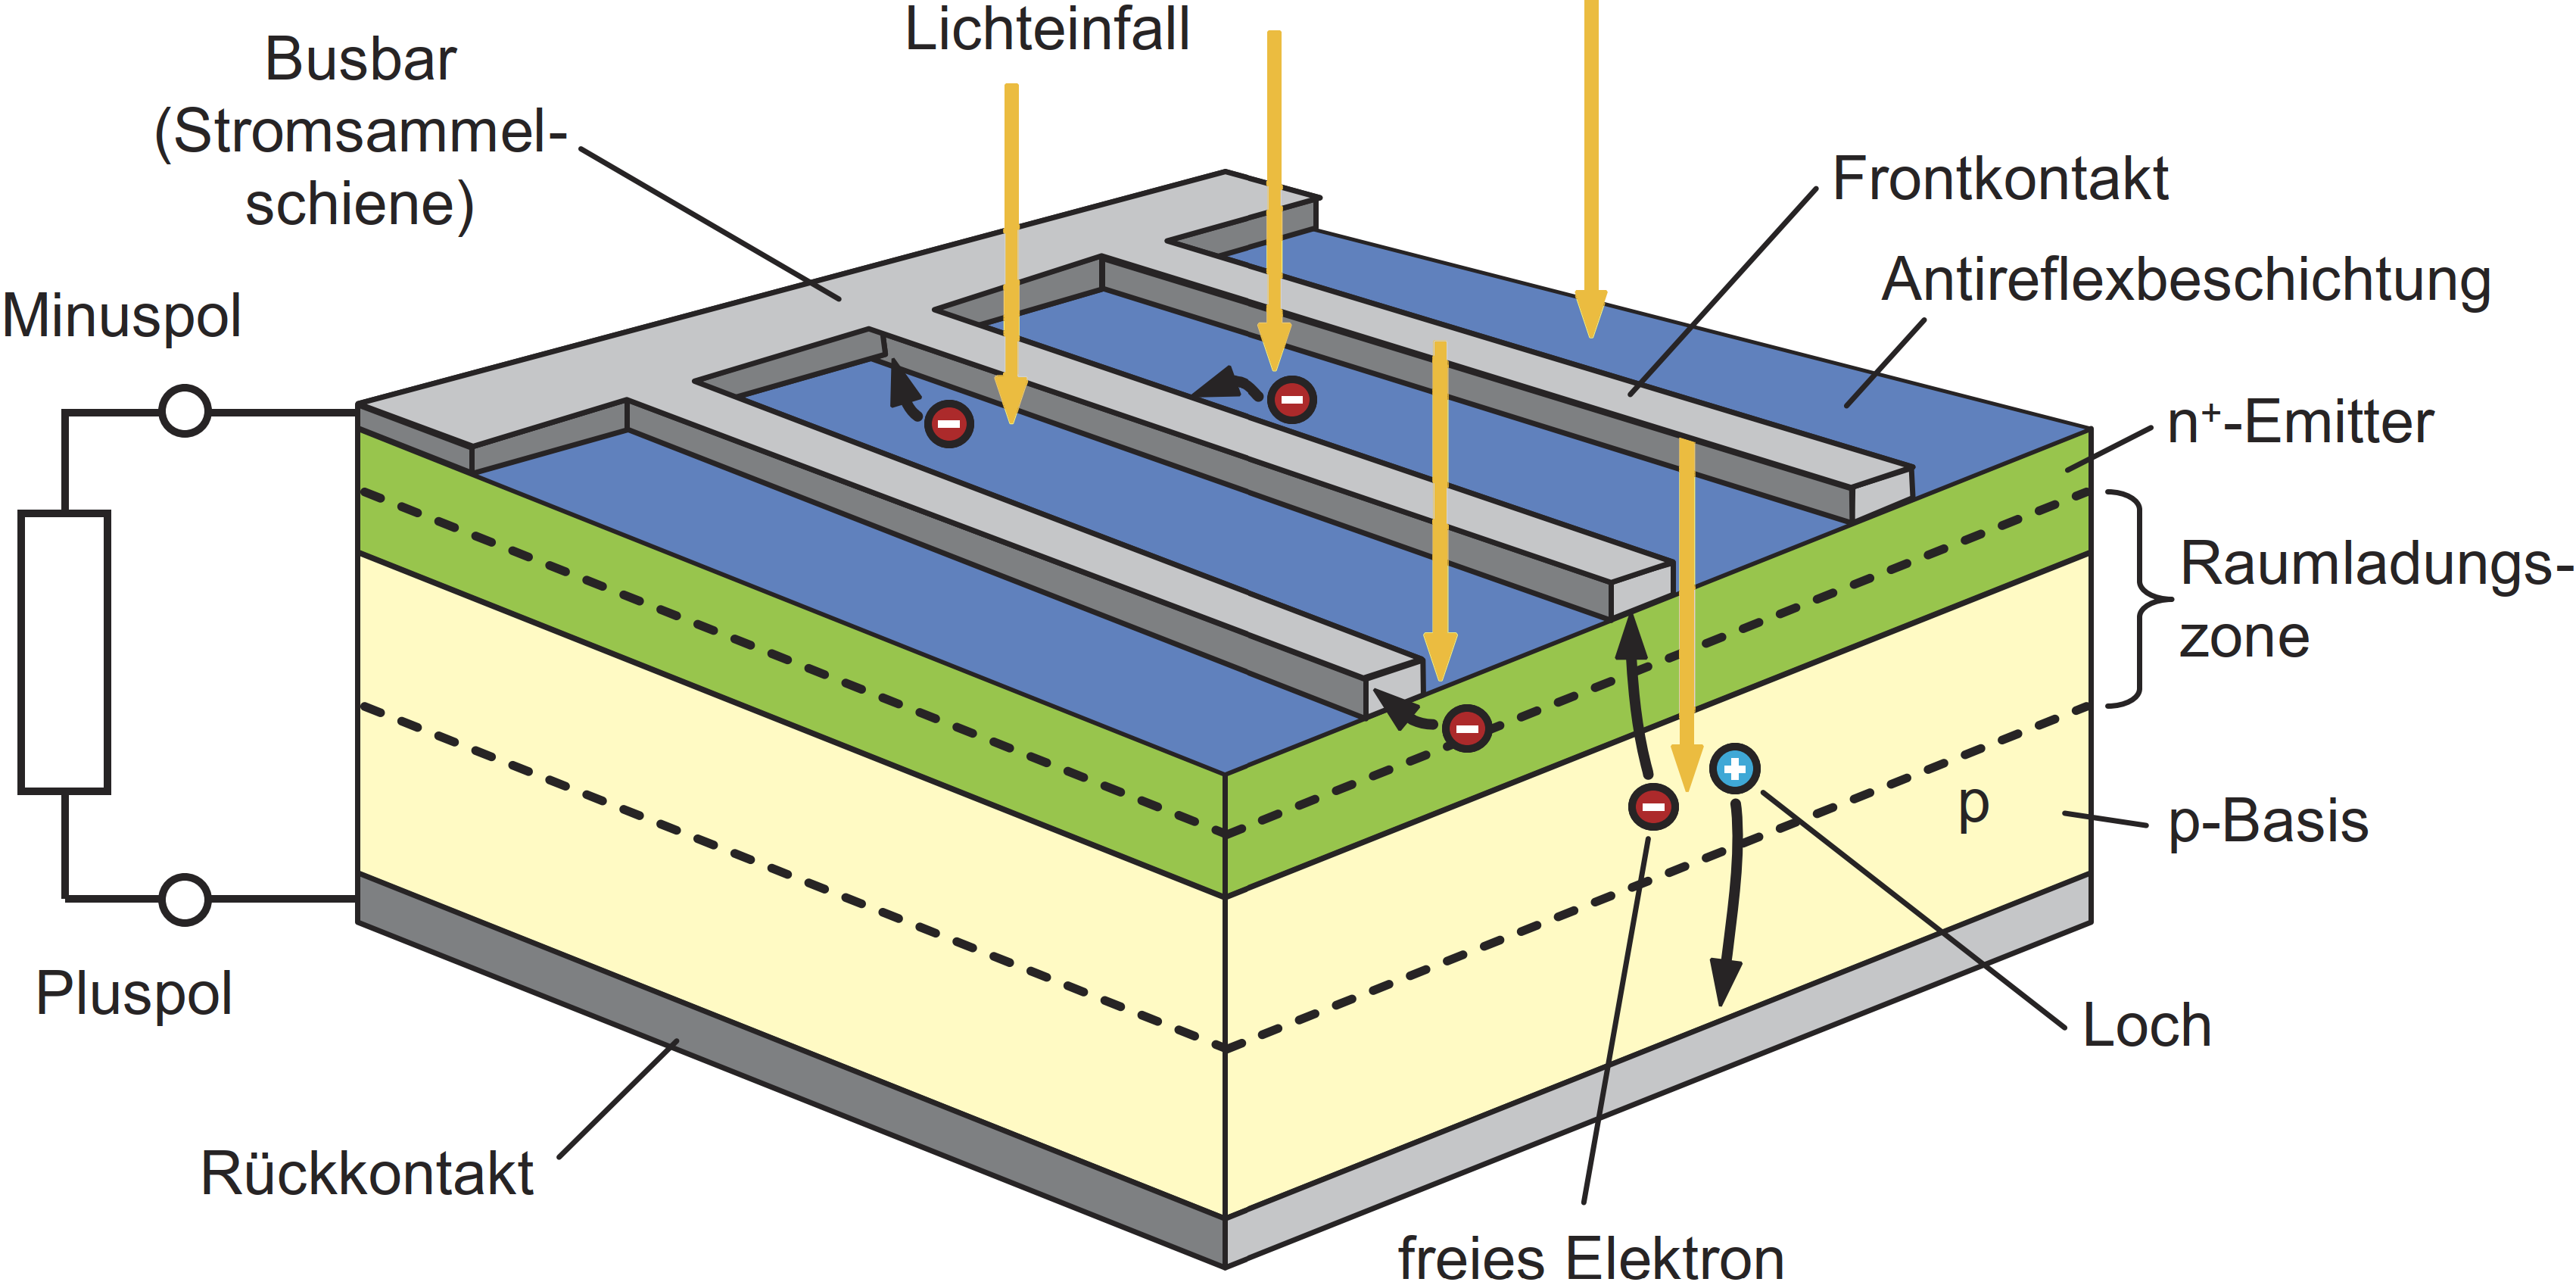
\includegraphics[width=0.99\linewidth]{images/Aufbau_Solarzelle.png}


\subsection{Aufbau Solarzelle}
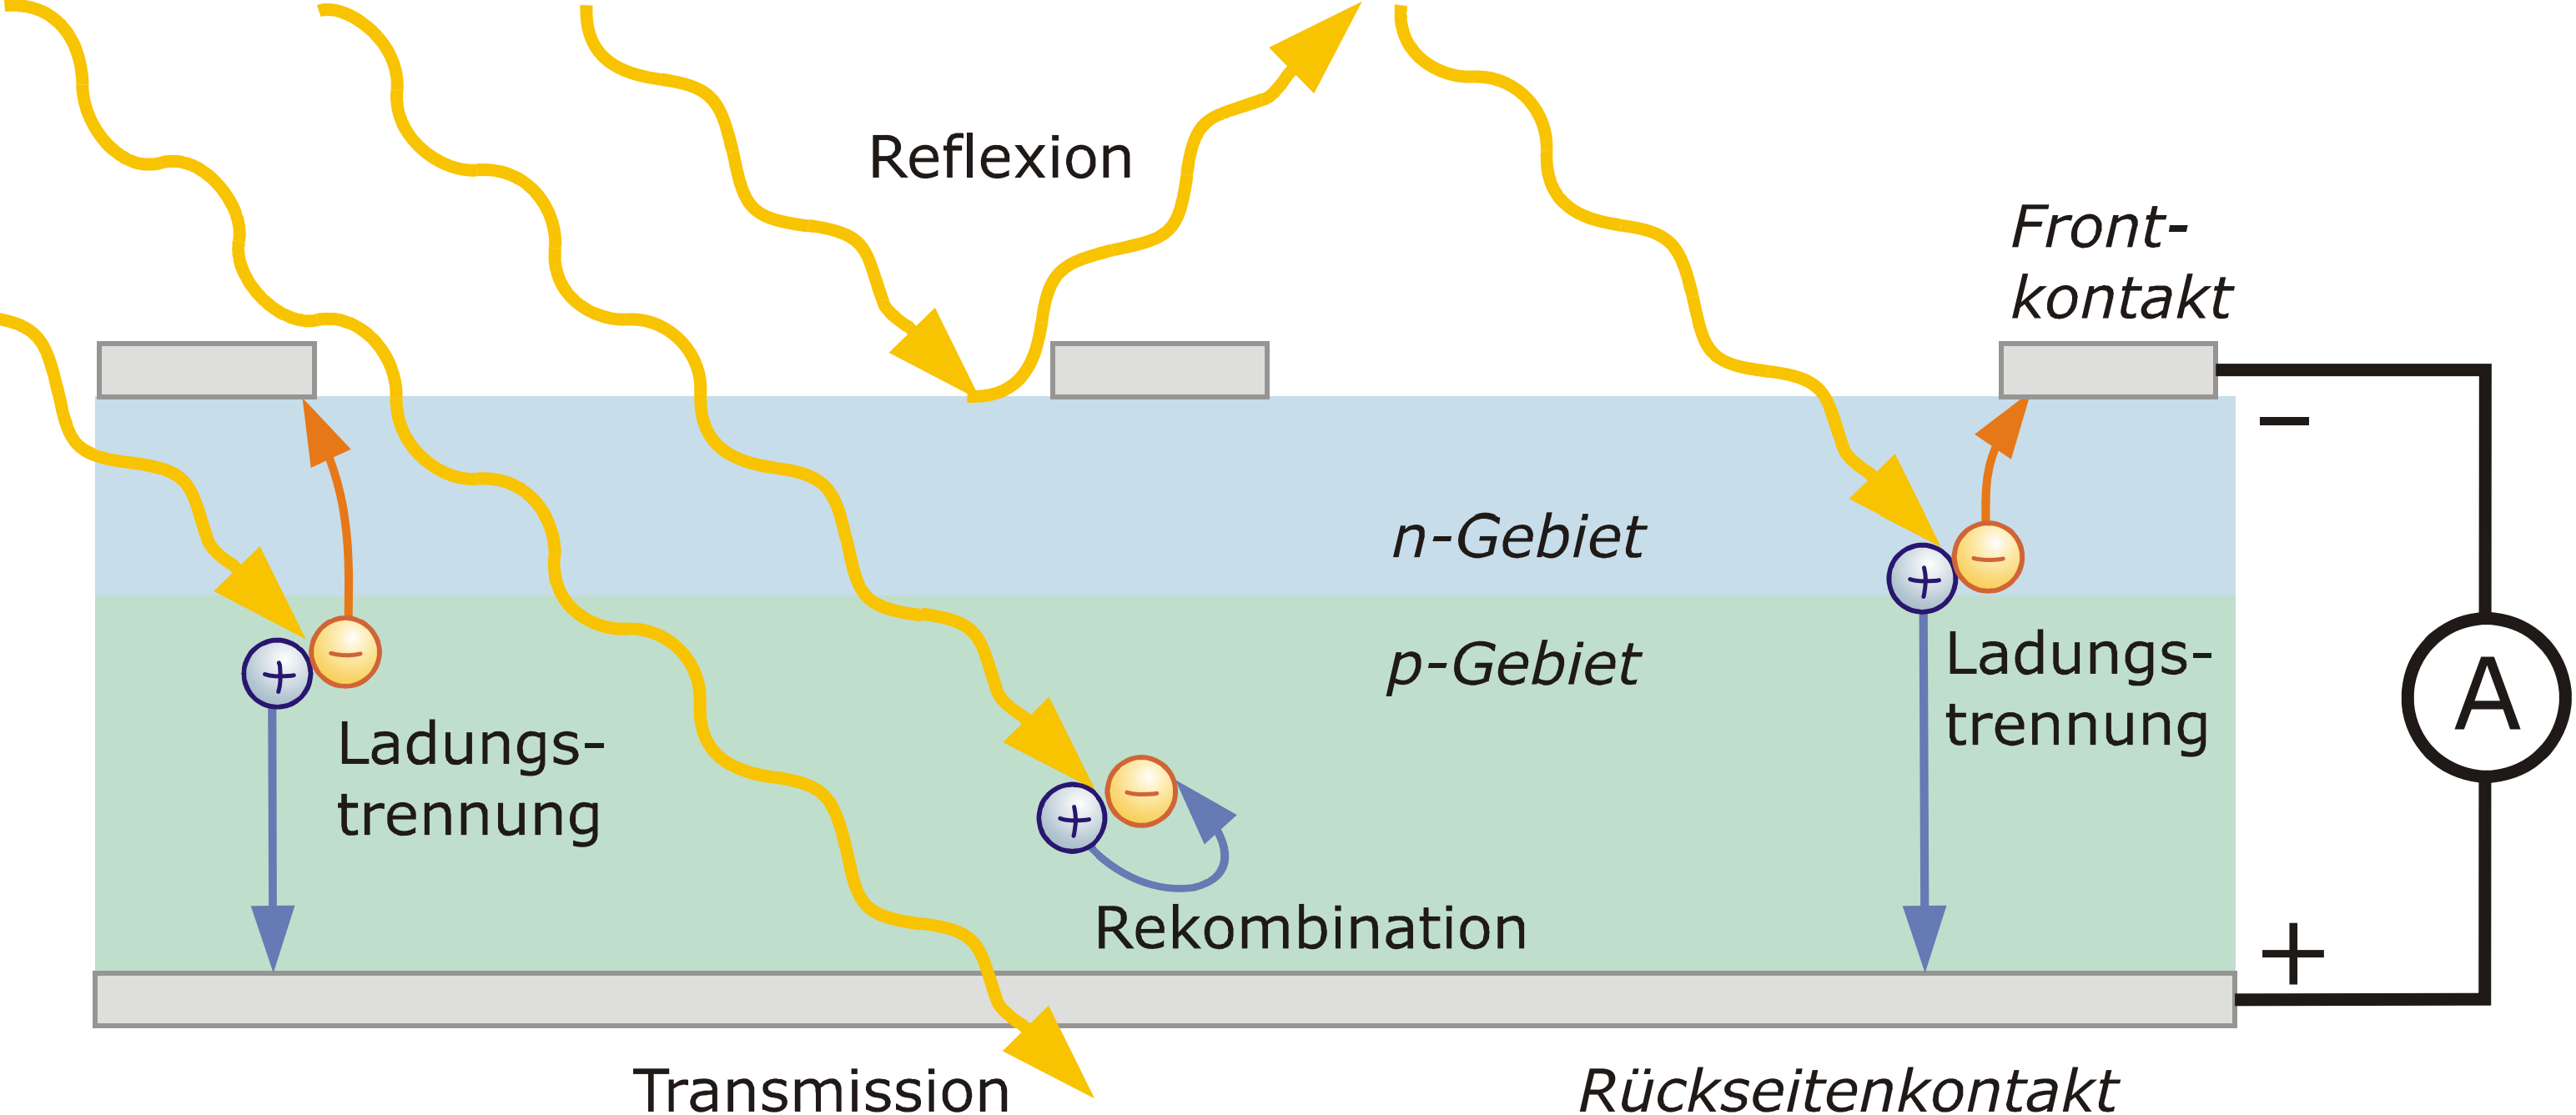
\includegraphics[width=0.99\linewidth]{images/Solarzelle_bei_Bestrahlung.png}


\subsection{Quantenwirkungsgrad}

\subsubsection{Externer Quantenwirkungsgrad}
Die externe Quanteneffizienz $\eta_{\text{Ext}}$ beschreibt das Verhältnis von erzeugten nutzbaren Elektron-Loch-Paaren zu den einfallenden Photonen:

$\boxed{\eta_{\text{Ext}} = \frac{N_{ELP}}{N_{Ph}}}$

\vspace{0.25cm}

\renewcommand{\arraystretch}{1.2} % Erhöht Zeilenhöhe für bessere Lesbarkeit
\begin{tabular}{@{} l p {5cm} l @{}}
    $[\eta_{\text{Ext}}]$   & Externe Quanteneffizienz              \dotfill & $-$ \\
    $[N_{ELP}]$         & Anzahl nutzbarer Elektron-Loch-Paare  \dotfill & $-$ \\
    $[N_{Ph}]$          & Anzahl auftreffender Photonen         \dotfill & $-$ \\
\end{tabular}

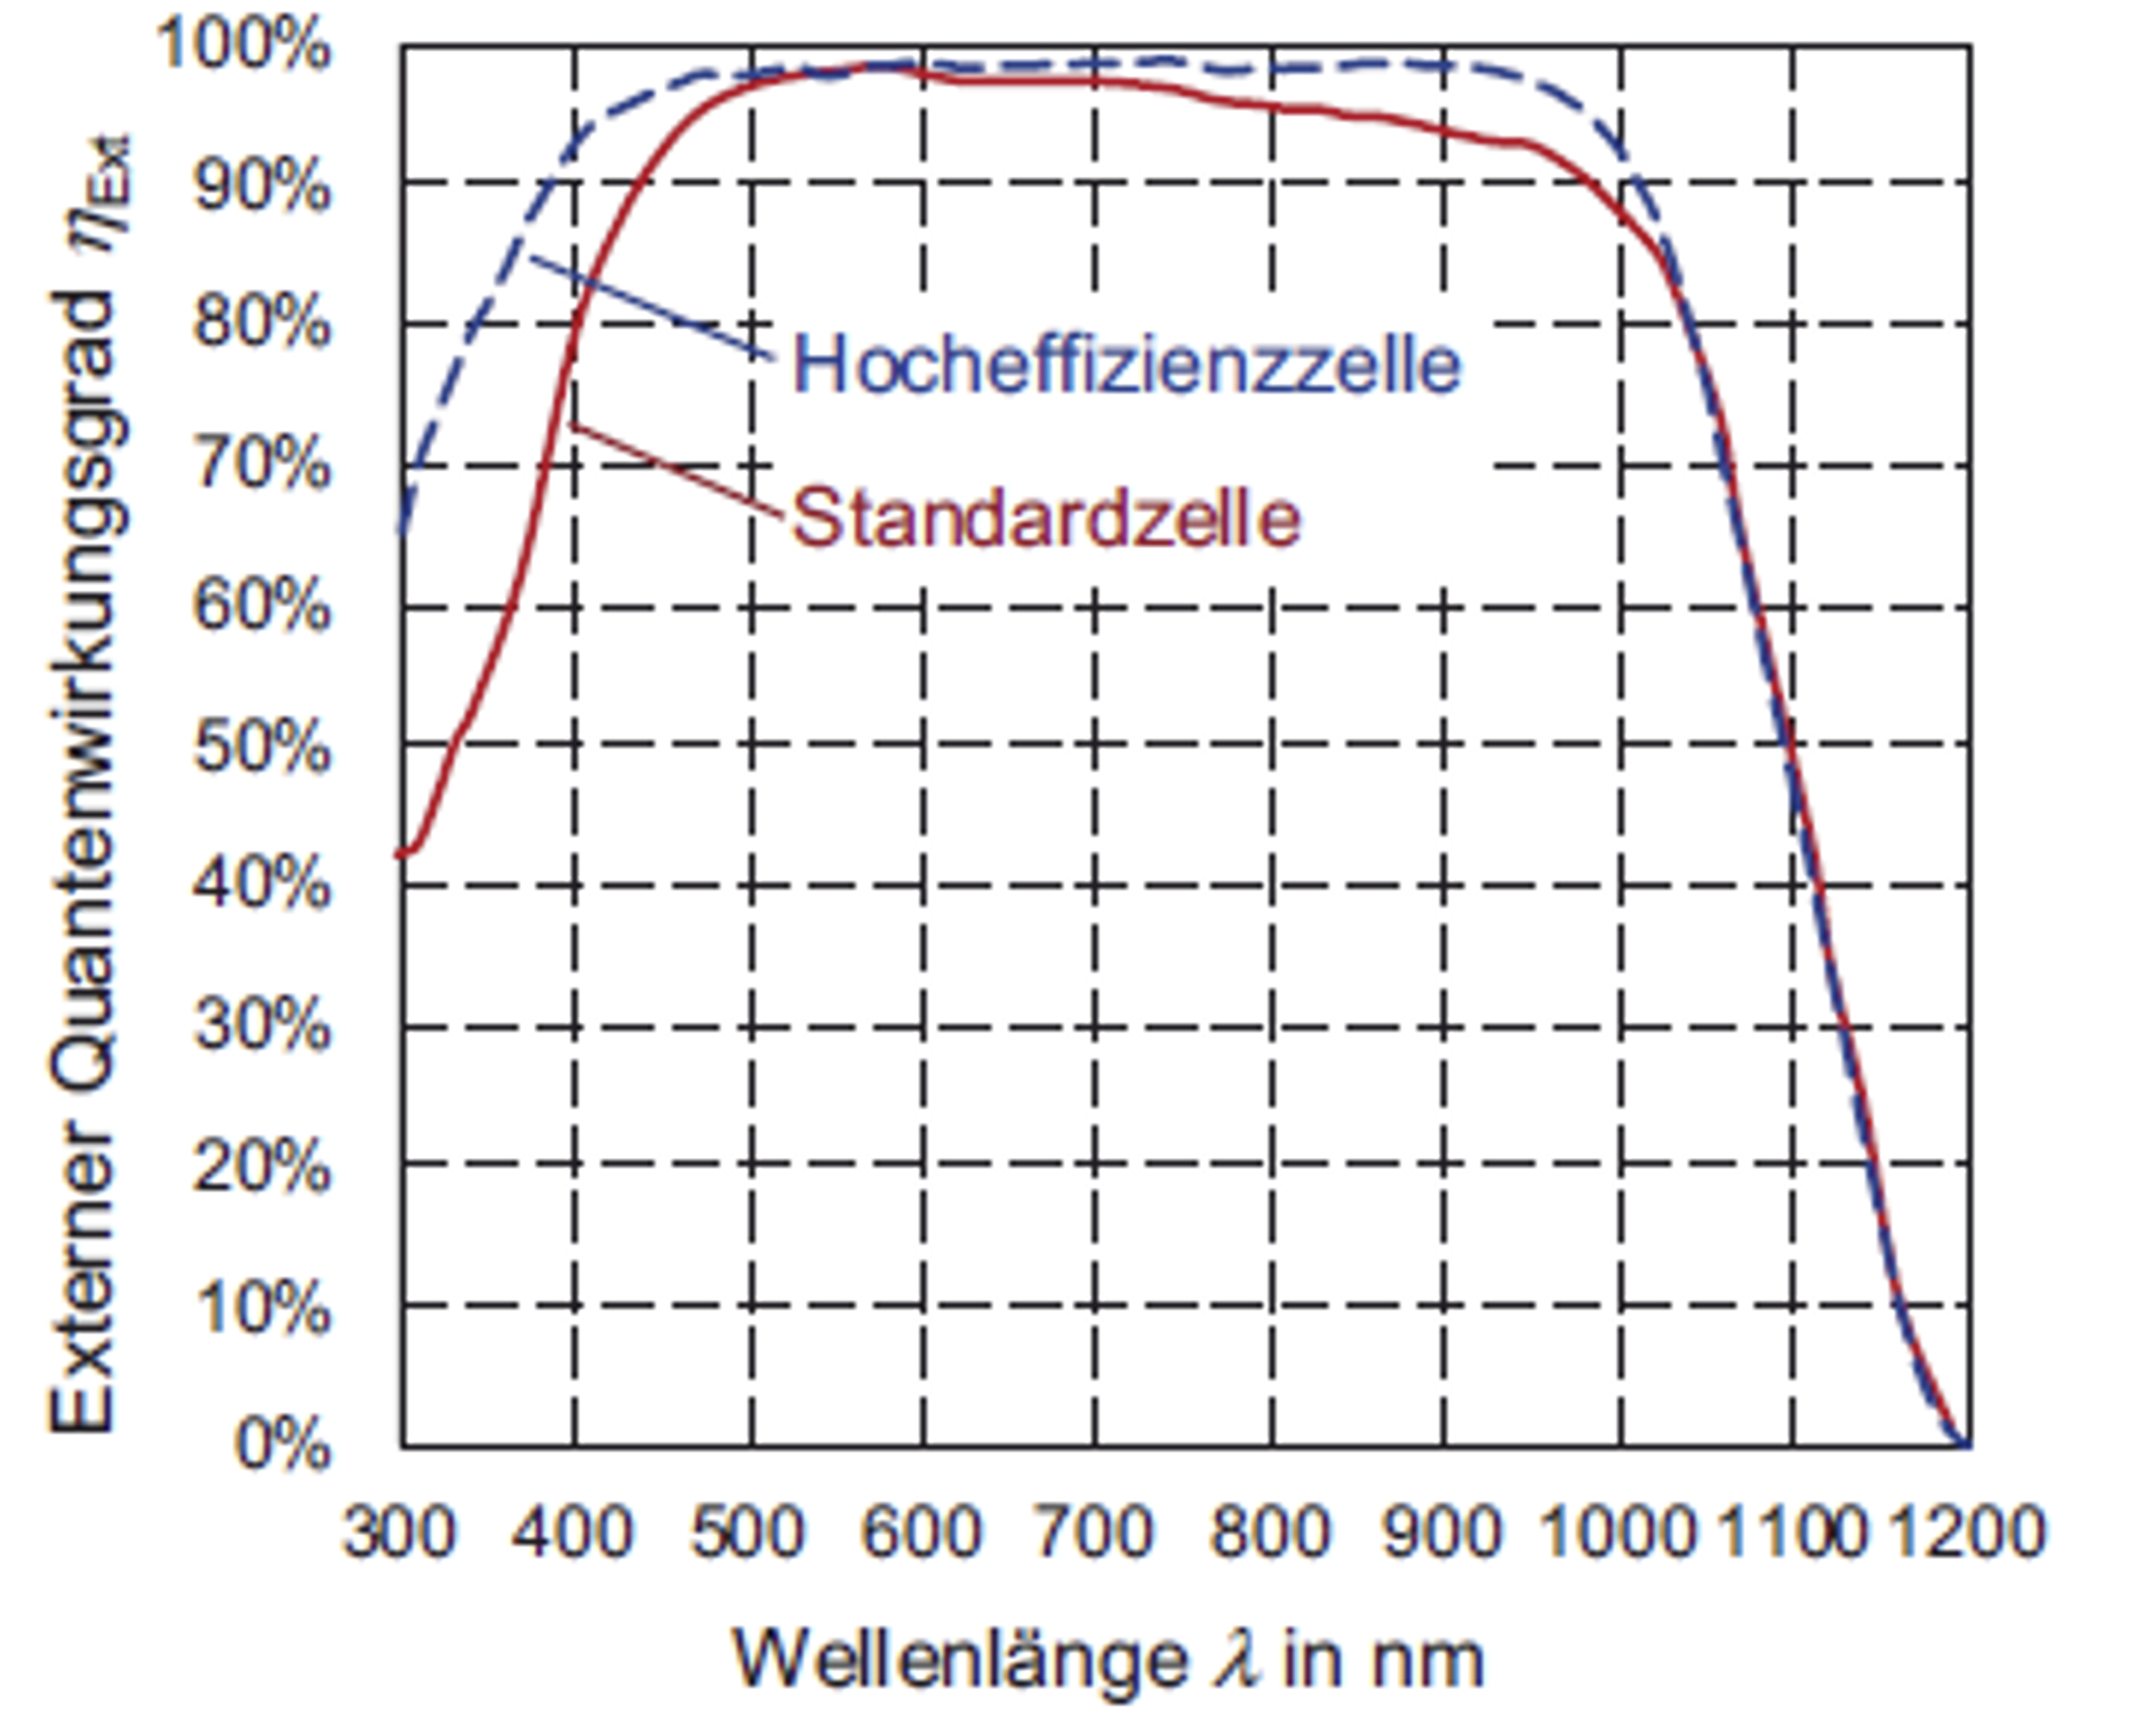
\includegraphics[width=0.55\linewidth]{images/Quantenwirkungsgrad.png}


\subsubsection{Interner Quantenwirkungsgrad}
Der interne Quantenwirkungsgrad $\eta_{\text{Int}}$ (ohne durch Reflexion verursachte Verluste) berechnet sich wie folgt:

$\boxed{\eta_{\text{Int}} = \frac{\eta_{\text{Ext}}}{1 - R}}$

\vspace{0.25cm}

\renewcommand{\arraystretch}{1.2} % Erhöht Zeilenhöhe für bessere Lesbarkeit
\begin{tabular}{@{} l p {5cm} l @{}}
    $[\eta_{\text{Int}}]$   & Interner Quantenwirkungsgrad      \dotfill & $-$ \\
    $[\eta_{\text{Ext}}]$   & Externer Quantenwirkungsgrad      \dotfill & $-$ \\
    $[R]$                   & Reflexionsfaktor                  \dotfill & $-$ \\
\end{tabular}

\subsection{Spektrale Empfindlichkeit $S(\lambda)$}

Die spektrale Empfindlichkeit $S(\lambda)$ gibt an, welcher Photostrom bei Auftreffen einer bestimmten optischen Leistung erzeugt wird:


$\boxed{
S(\lambda) 
= \frac{I_{\text{Ph}}}{P_{\text{Opt}}}
}$  $\boxed{
S(\lambda) 
= \frac{\frac{Q}{\Delta t}}{\frac{W_{\text{Opt}}}{\Delta t}}
}$  $\boxed{
S(\lambda) 
= \frac{q}{h \cdot f} \cdot \eta_{\text{Ext}}
}$  $\boxed{
S(\lambda) 
= \frac{q}{h \cdot c_0} \cdot \lambda \cdot \eta_{\text{Ext}}
}$

\vspace{0.25cm}

Mit eingesetzten Konstanten ergibt sich:\\
$\boxed{
S(\lambda) 
= \frac{\lambda}{1,24 \mu m} \cdot \eta_{\text{Ext}}
}$

\vspace{0.25cm}

\renewcommand{\arraystretch}{1.2} % Erhöht Zeilenhöhe für bessere Lesbarkeit
\begin{tabular}{@{} l p {6cm} l @{}}
    $[S(\lambda)]$        & Spektrale Empfindlichkeit  \dotfill & $\frac{A}{W}$ \\
    $[I_{\text{Ph}}]$     & Photostrom                \dotfill & $A$ \\
    $[P_{\text{Opt}}]$    & Optische Leistung       \dotfill & $W$ \\
    $[Q]$                 & Elektrische Ladung       \dotfill & $C$ \\
    $[W_{\text{Opt}}]$    & Optische Energie       \dotfill & $J$ \\
    $[q]$                 & Elementarladung           \dotfill & $C$ \\
    $[h]$                 & Planck-Konstante          \dotfill & $J \cdot s$ \\
    $[f]$                 & Frequenz                  \dotfill & $Hz$ \\
    $[c_0]$               & Lichtgeschwindigkeit      \dotfill & $\frac{m}{s}$ \\
    $[\lambda]$           & Wellenlänge               \dotfill & $m$ \\
    $[\eta_{\text{Ext}}]$ & Externe Quanteneffizienz \dotfill  0.550.55& $-$ \\
\end{tabular}

\vspace{0.25cm}

\renewcommand{\arraystretch}{1.4} %Erhöht Zeilenhöhe für bessere Lesbarkeit 
\begin{tabular}{@{} l | l | l @{}} 
    \textbf{FZ} & \textbf{Bezeichnung} & \textbf{Wert der Konstanten} \\\hline 
    $q$ & Elementarladung                   & $1{,}602 \cdot 10^{-19} C$ \\ 
    $h$ & Planck-Konstante                  & $\approx 6{,}6 \cdot 10^{-34} W s^2$ \\ 
    $c$ & Lichtgeschwindigkeit im Vakuum    & $ \approx 3 \cdot 10^{8} \frac{m}{s}$ \\
\end{tabular}

\vspace{0.25cm}

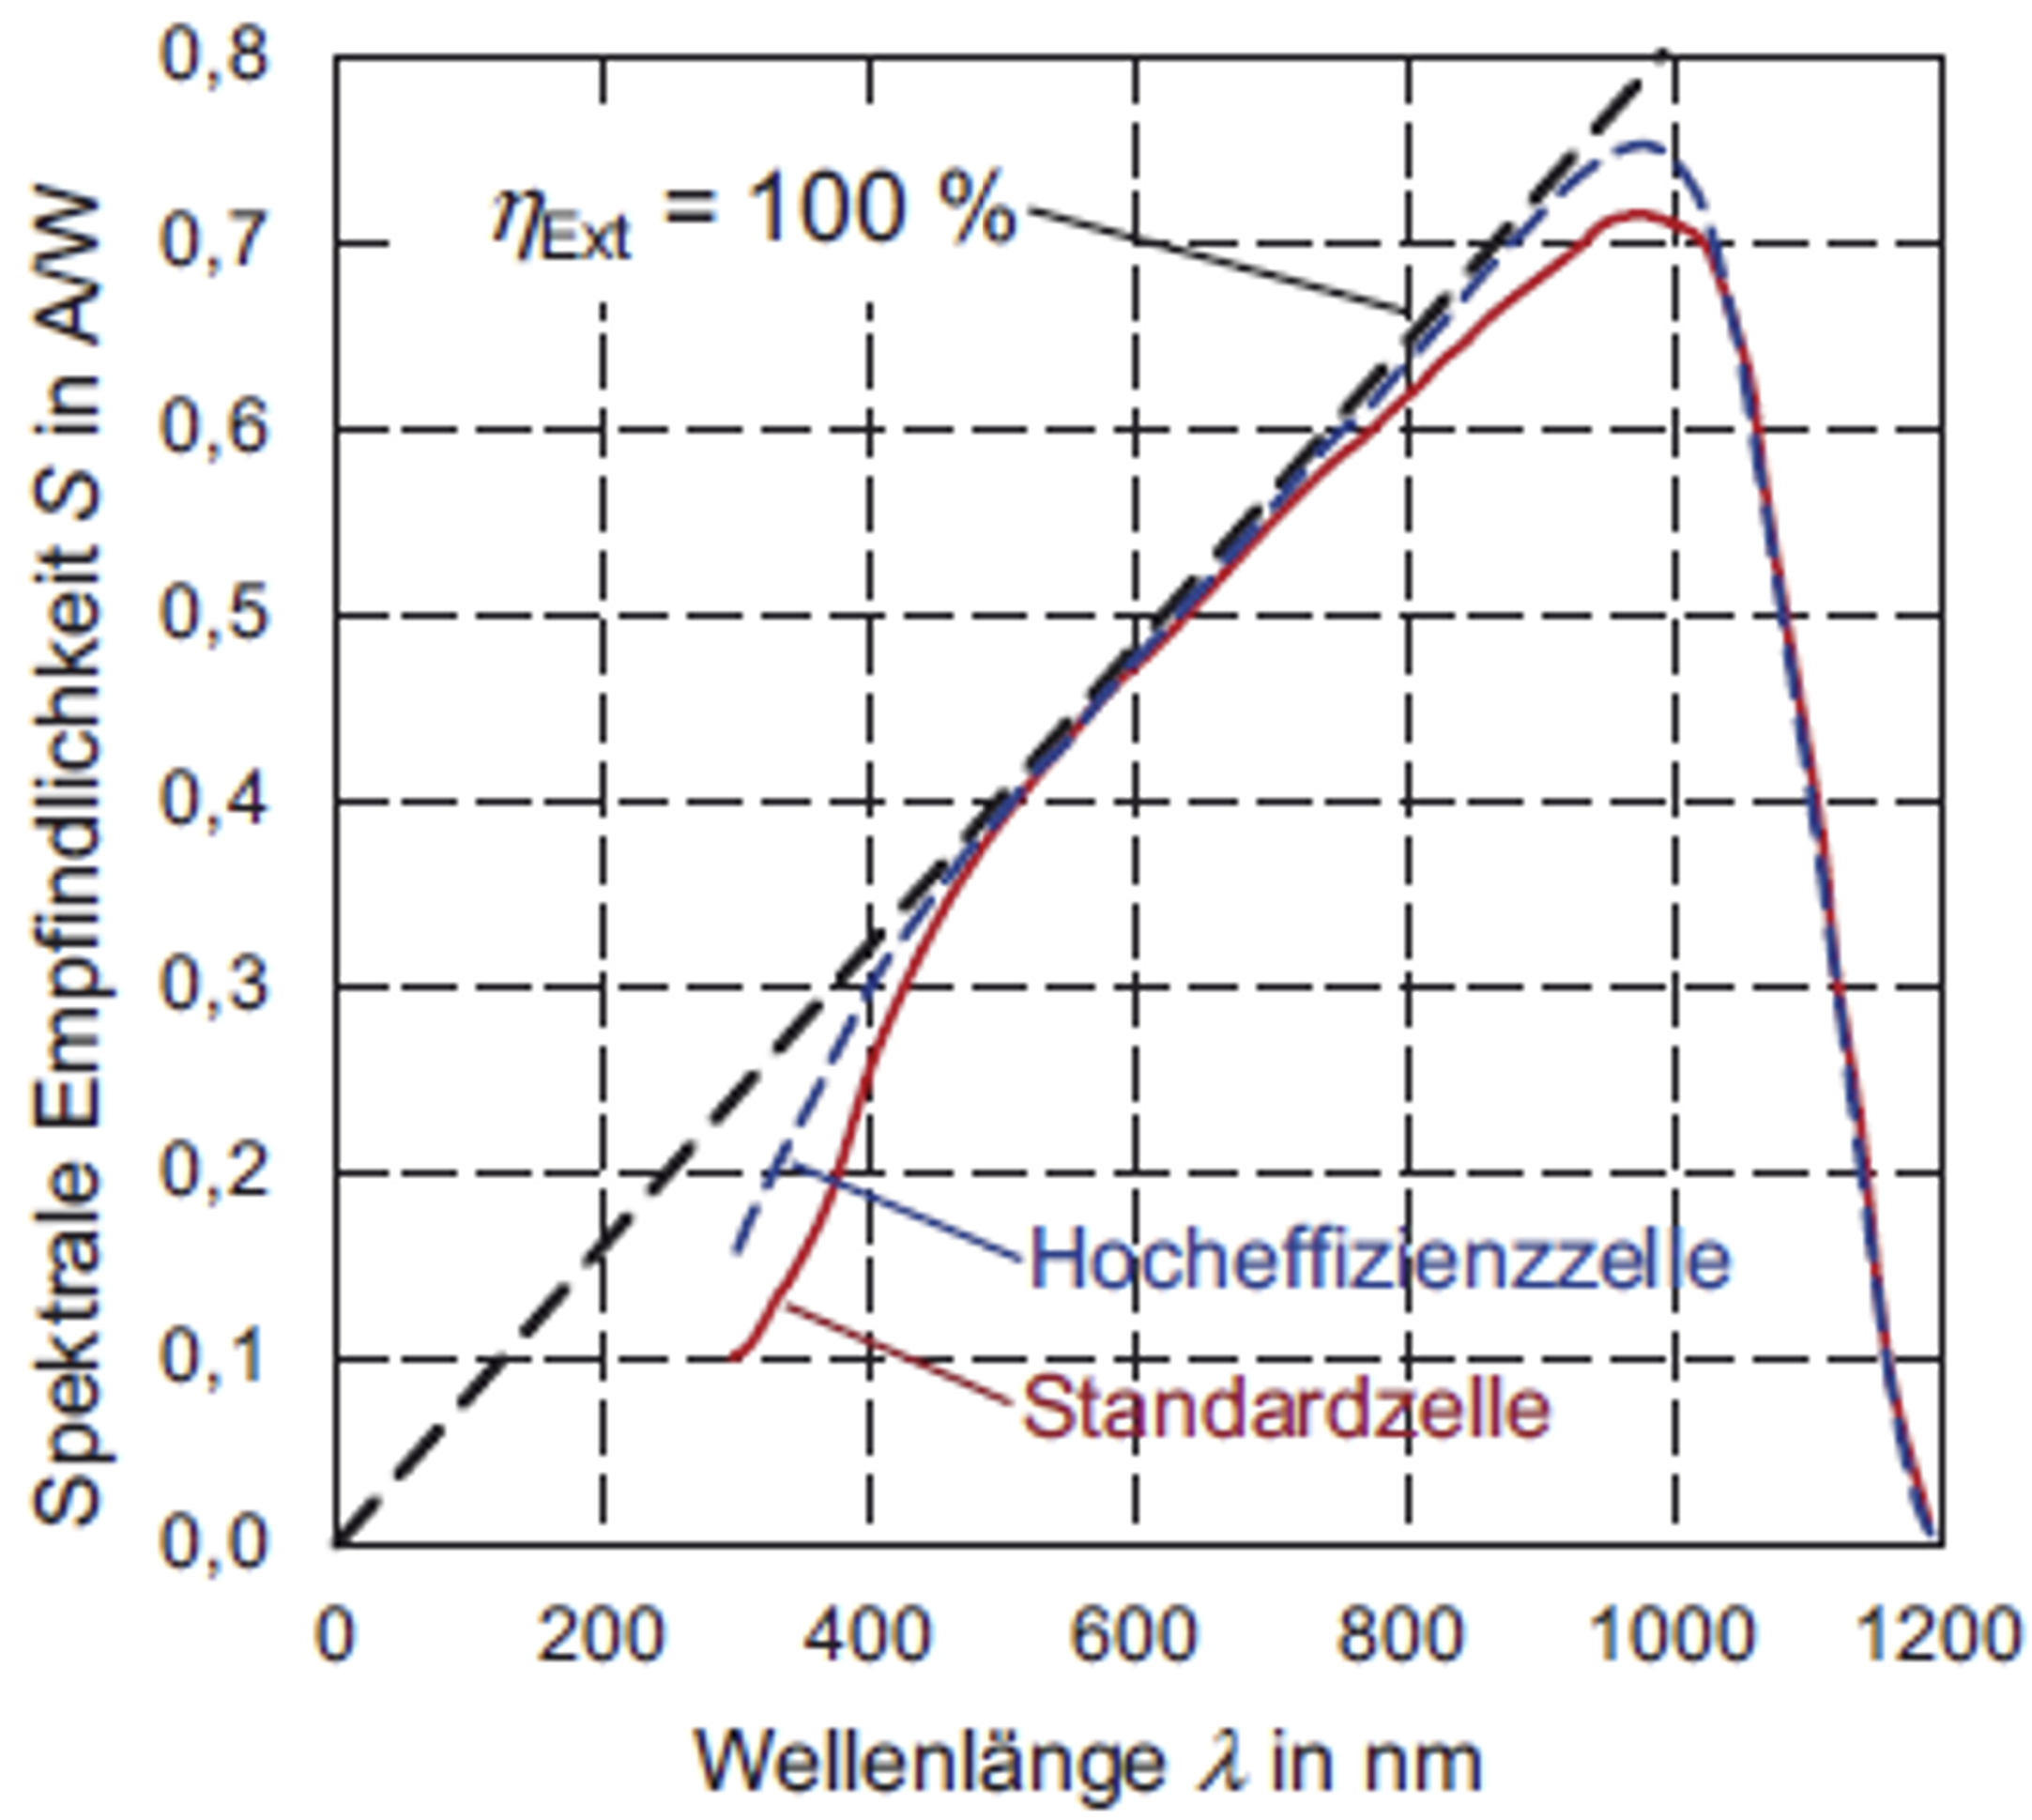
\includegraphics[width=0.55\linewidth]{images/Spektrale_Empfindlichkeit.png}

\newcolumn
\subsection{Verlustmechan. durch unpassende Energie der Photonen}

Eine grundsätzliche Beschränkung des Wirkungsgrads einer Solarzelle ergibt sich daraus, dass jedes Halbleitermaterial einen Bandabstand $\Delta W_G$ aufweist. 
Die Wellenlänge, bei der Licht gerade noch absorbiert wird, nennen wir die \textbf{Bandlückenwellenlänge} $\lambda_G$ mit

$\boxed{\lambda_G = \frac{h \cdot c}{\Delta W_G}}$

\vspace{0.25cm}

\renewcommand{\arraystretch}{1.2} % Erhöht Zeilenhöhe für bessere Lesbarkeit
\begin{tabular}{@{} l p {6cm} l @{}}
    $[\lambda_G]$    & Bandlückenwellenlänge (Grenzwellenlänge)  \dotfill & $m$ \\
    $[h]$            & Planck-Konstante                          \dotfill & $J \cdot s$ \\
    $[c]$            & Lichtgeschwindigkeit                      \dotfill & $\frac{m}{s}$ \\
    $[\Delta W_G]$   & Bandabstand (Bandlücke)                   \dotfill & $J$ \\
\end{tabular}

\vspace{0.25cm}

\begin{minipage}[t]{0.48\columnwidth}
    \myul{\textbf{$\lambda > \lambda_G$ : Durchstrahlung}}\\
    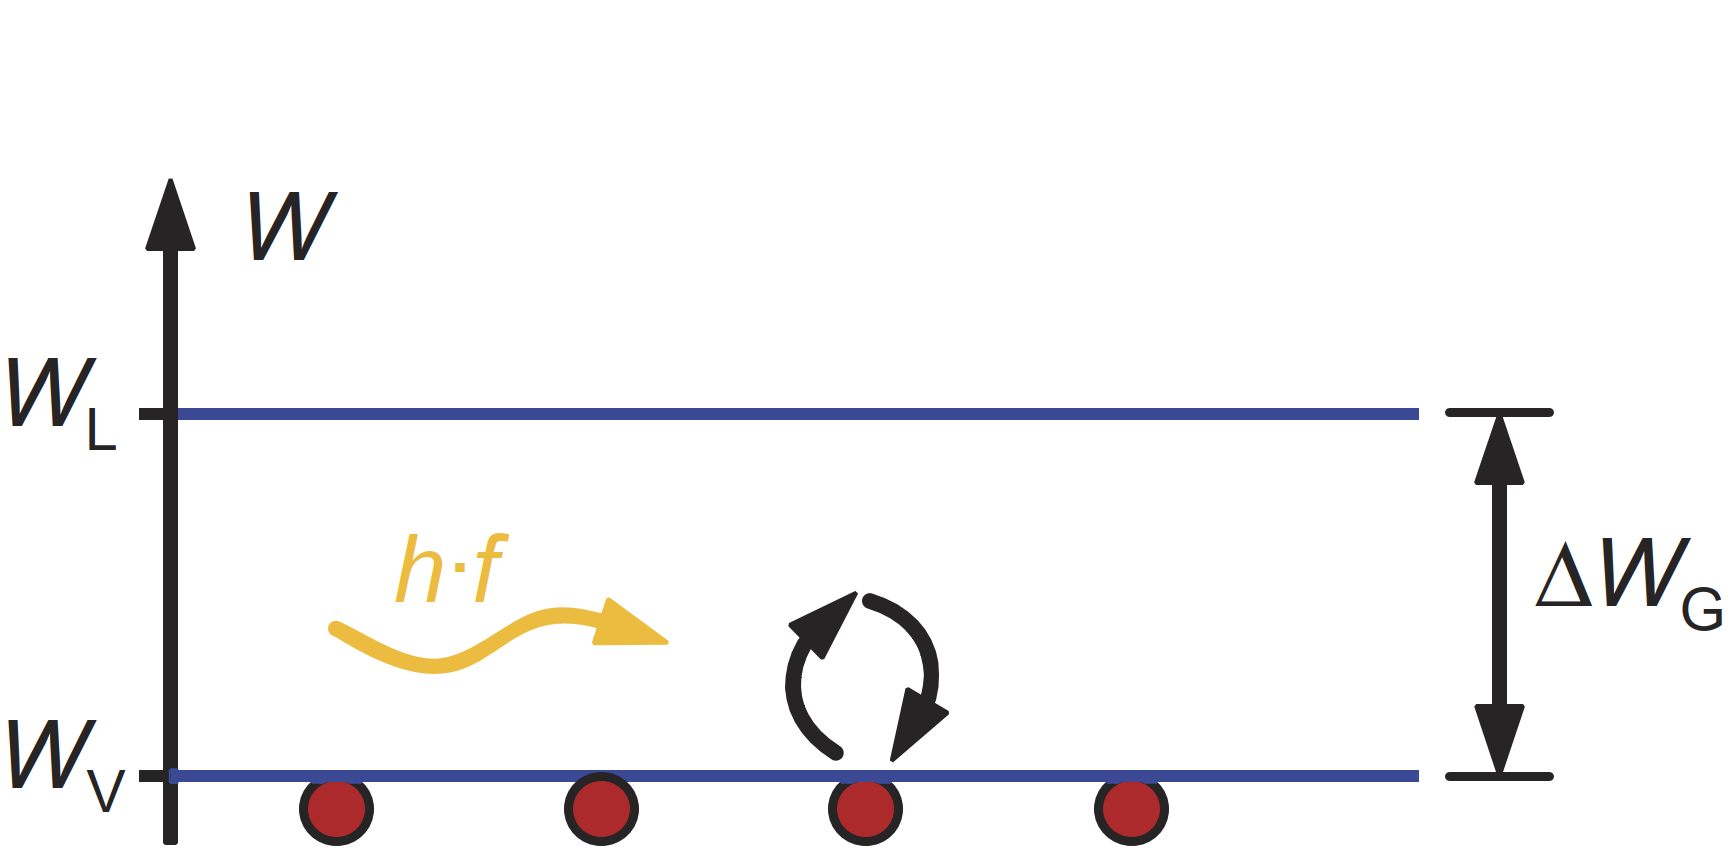
\includegraphics[width=0.9\columnwidth]{images/Spektraler_Wirkungsgrad_Durchstrahlung.png}
\end{minipage}
\hfill
\begin{minipage}[t]{0.48\columnwidth}
    \myul{\textbf{$\lambda < \lambda_G$ : Thermalisierung}}\\
    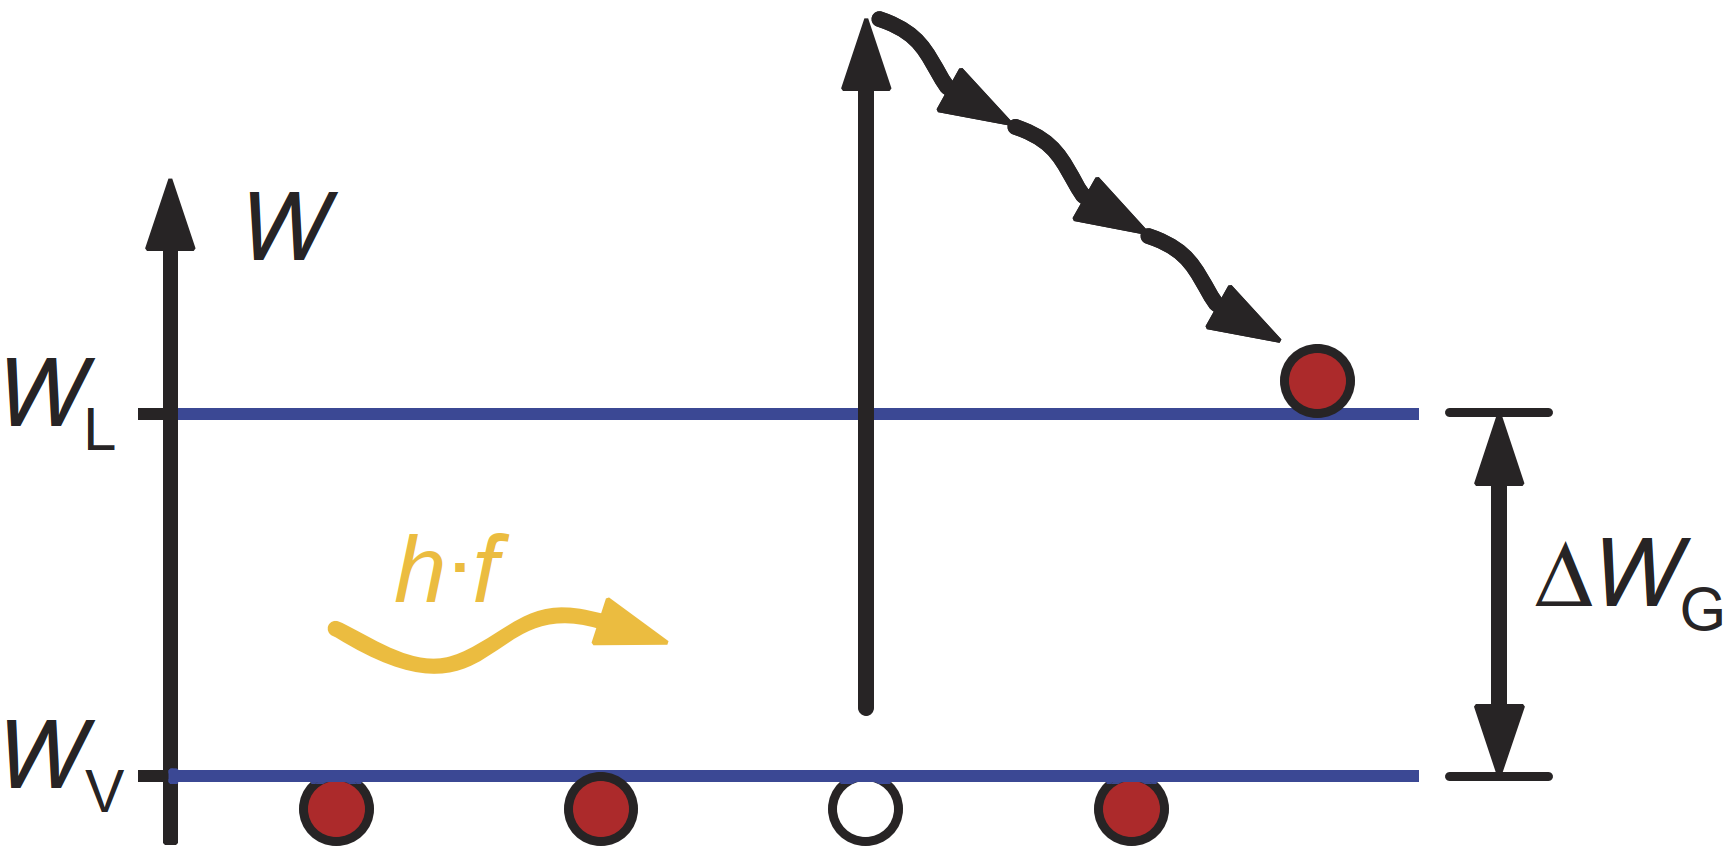
\includegraphics[width=0.9\columnwidth]{images/Spektraler_Wirkungsgrad_Thermalisierung.png}
\end{minipage}

\vspace{0.25cm}

\myul{\textbf{Durchstrahlung}} bezeichnet den Verlustmechanismus, bei dem Photonen mit zu geringer Energie die Solarzelle durchqueren, ohne absorbiert zu werden.\\
\myul{\textbf{Thermalisierung}} beschreibt den Energieverlust, bei dem Photonen mit zu hoher Energie nur einen Teil ihrer Energie an Elektronen abgeben, während die überschüssige Energie als Wärme verloren geht.


\subsection{Spektrale Verluste}
\begin{center}
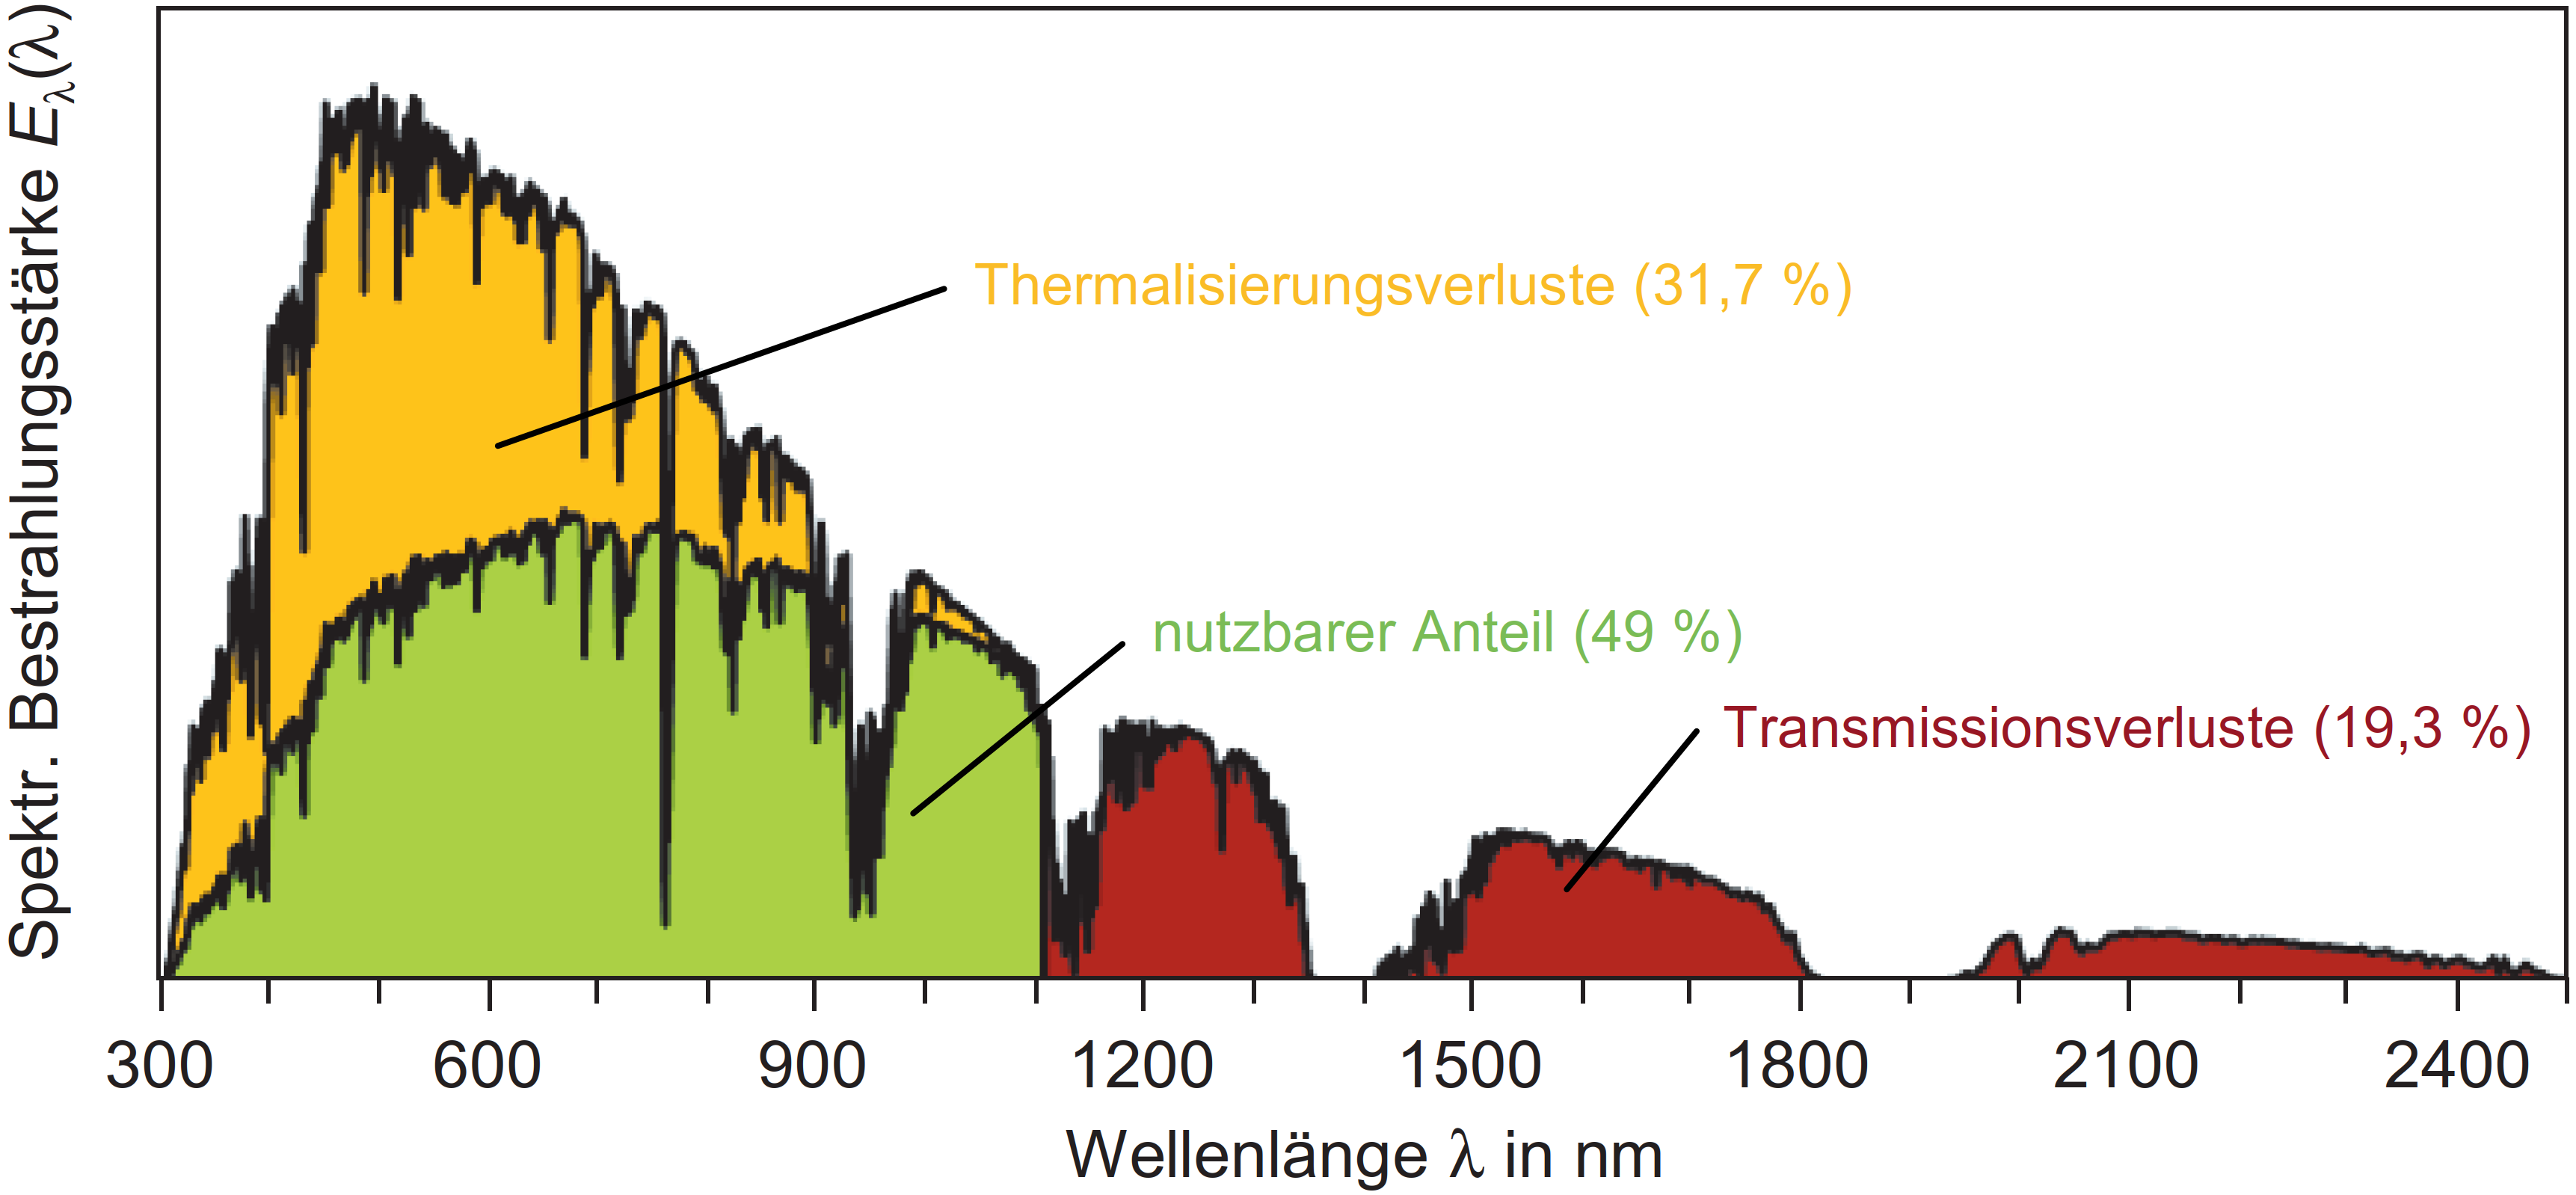
\includegraphics[width=0.95\columnwidth]{images/Spektrale_Verluste.png}
\end{center}


\subsection{Spektrale Wirkungsgrad idealer Solarzelle}
Der \textbf{theoretisch maximal mögliche Wirkungsgrad} für eine kristalline Siliziumsolarzelle liegt bei
ca. $29\%$
\begin{center}
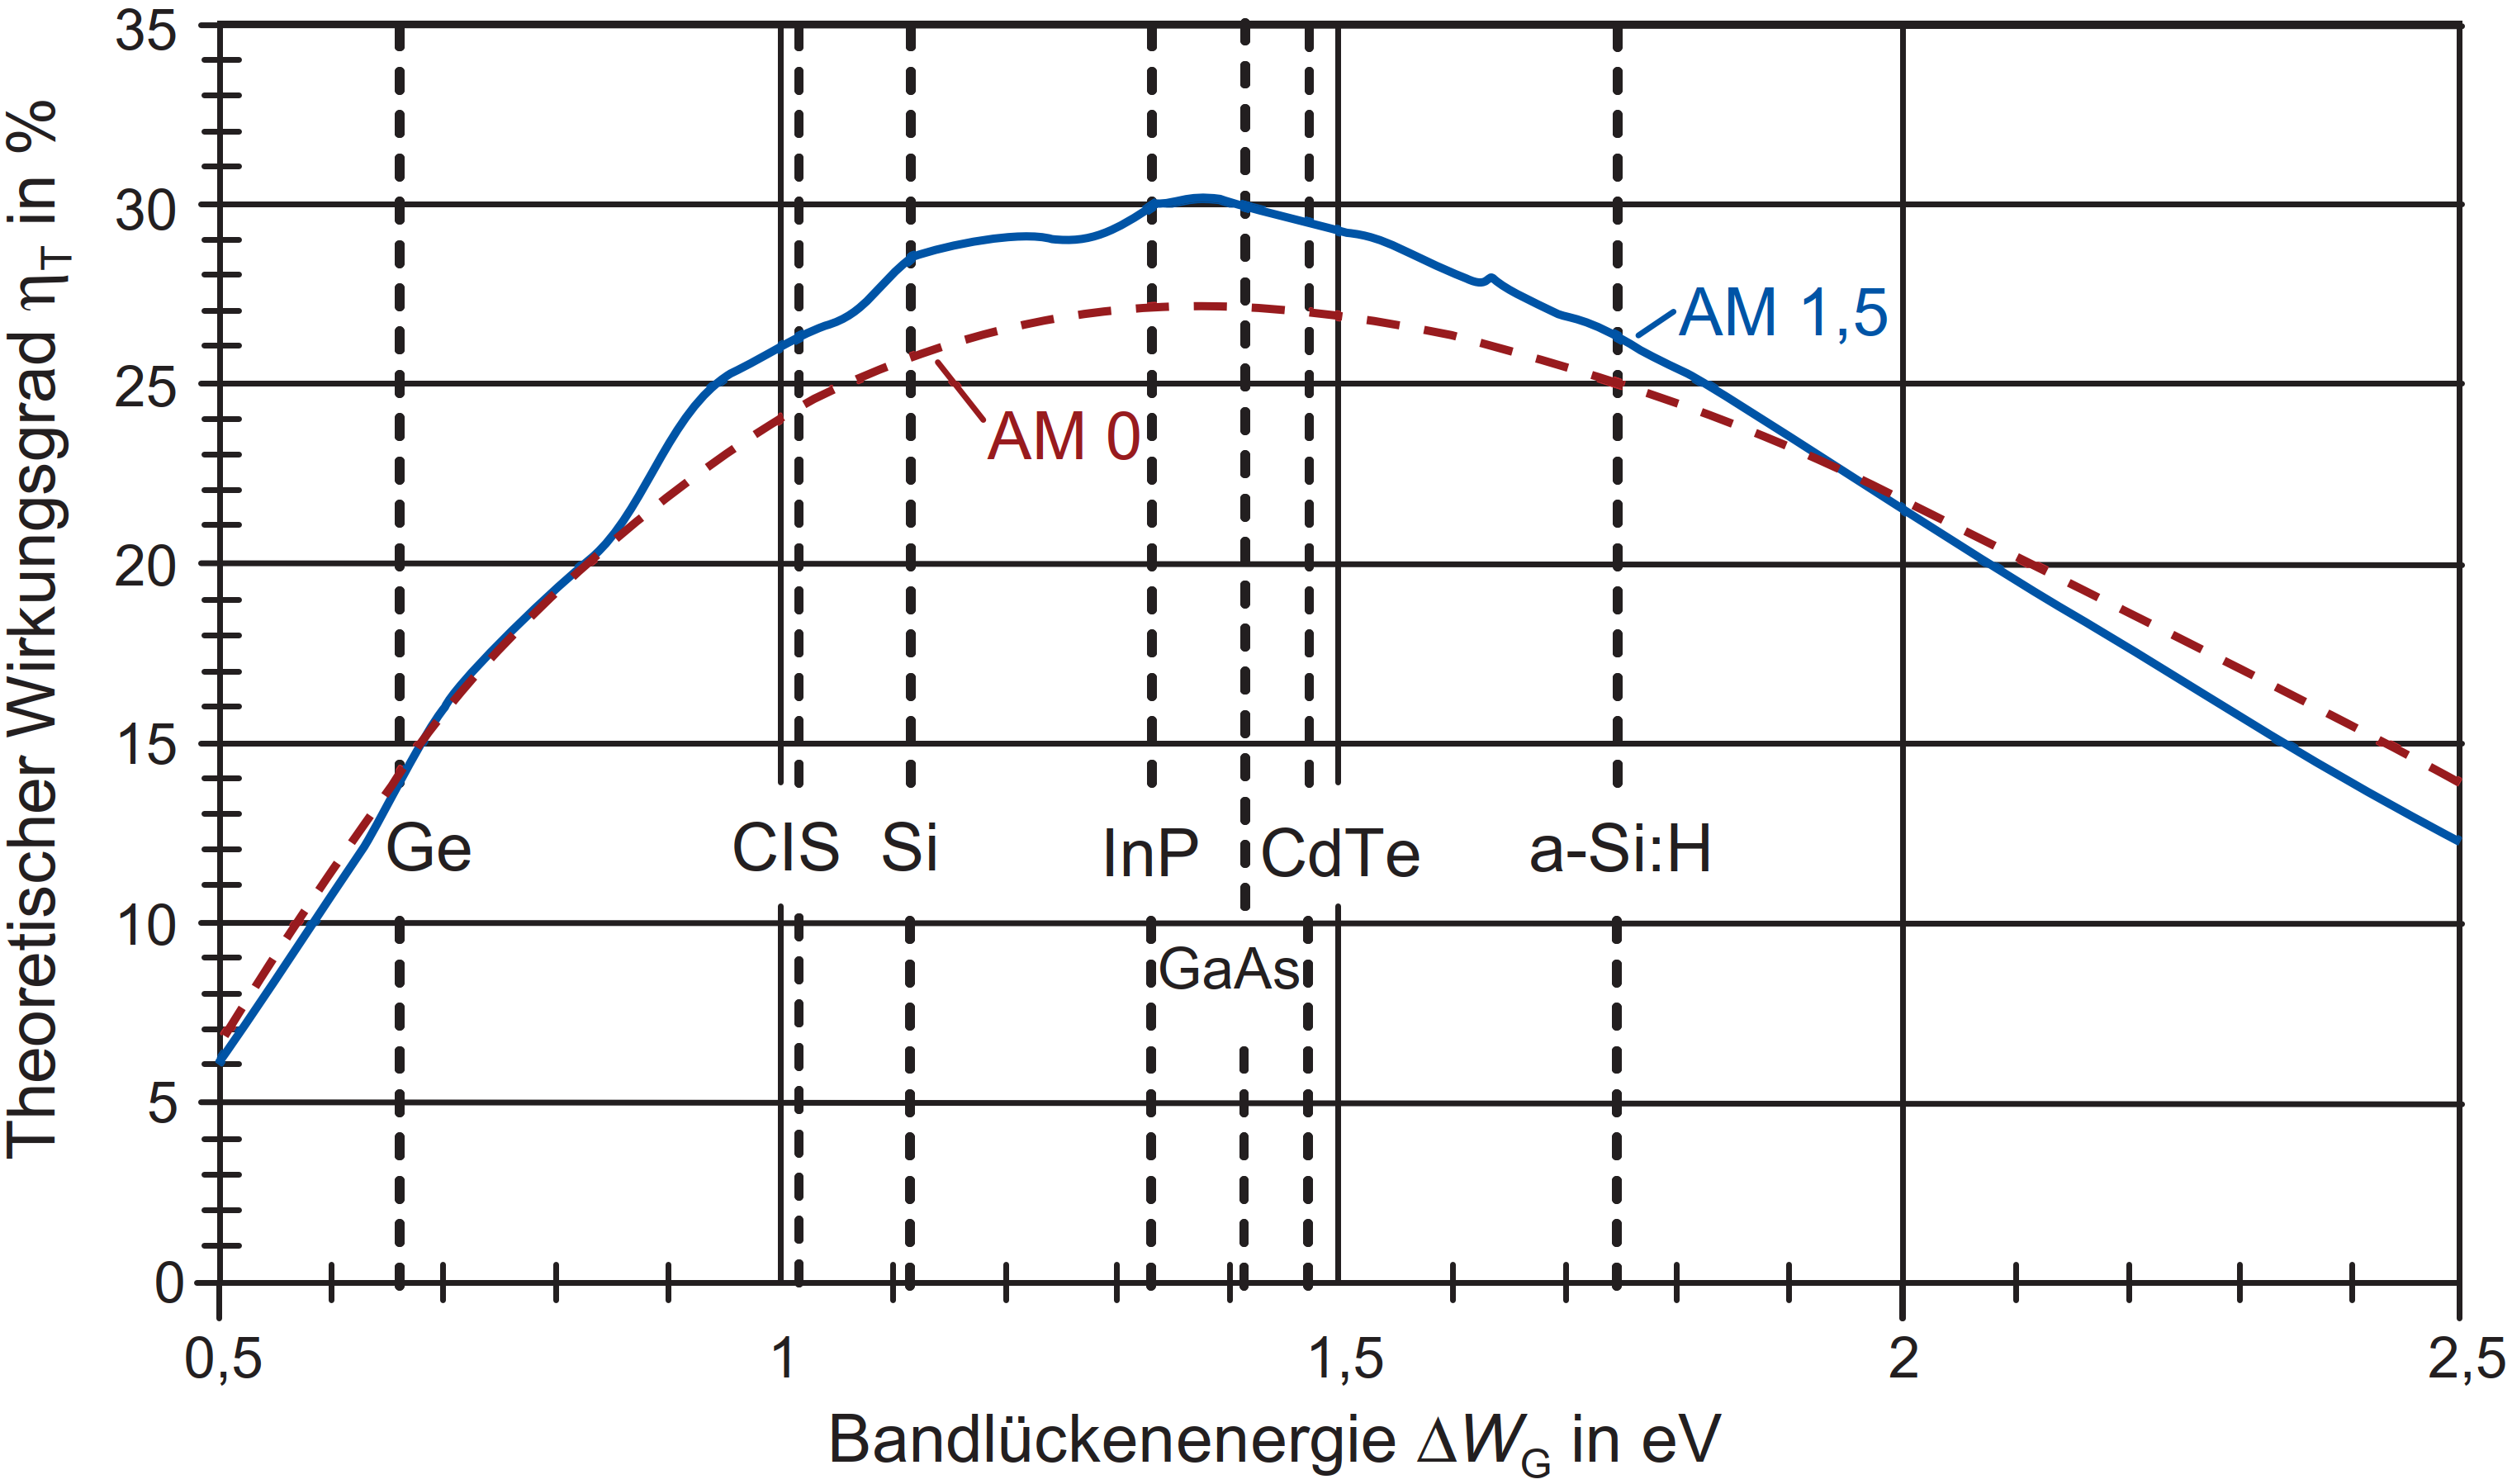
\includegraphics[width=0.95\columnwidth]{images/Spektraler_Wirkungsgrad_idealer_Solarzelle.png}
\end{center}


\subsection{Abschattung durch Kontaktfinger oder Busbars}
\begin{center}
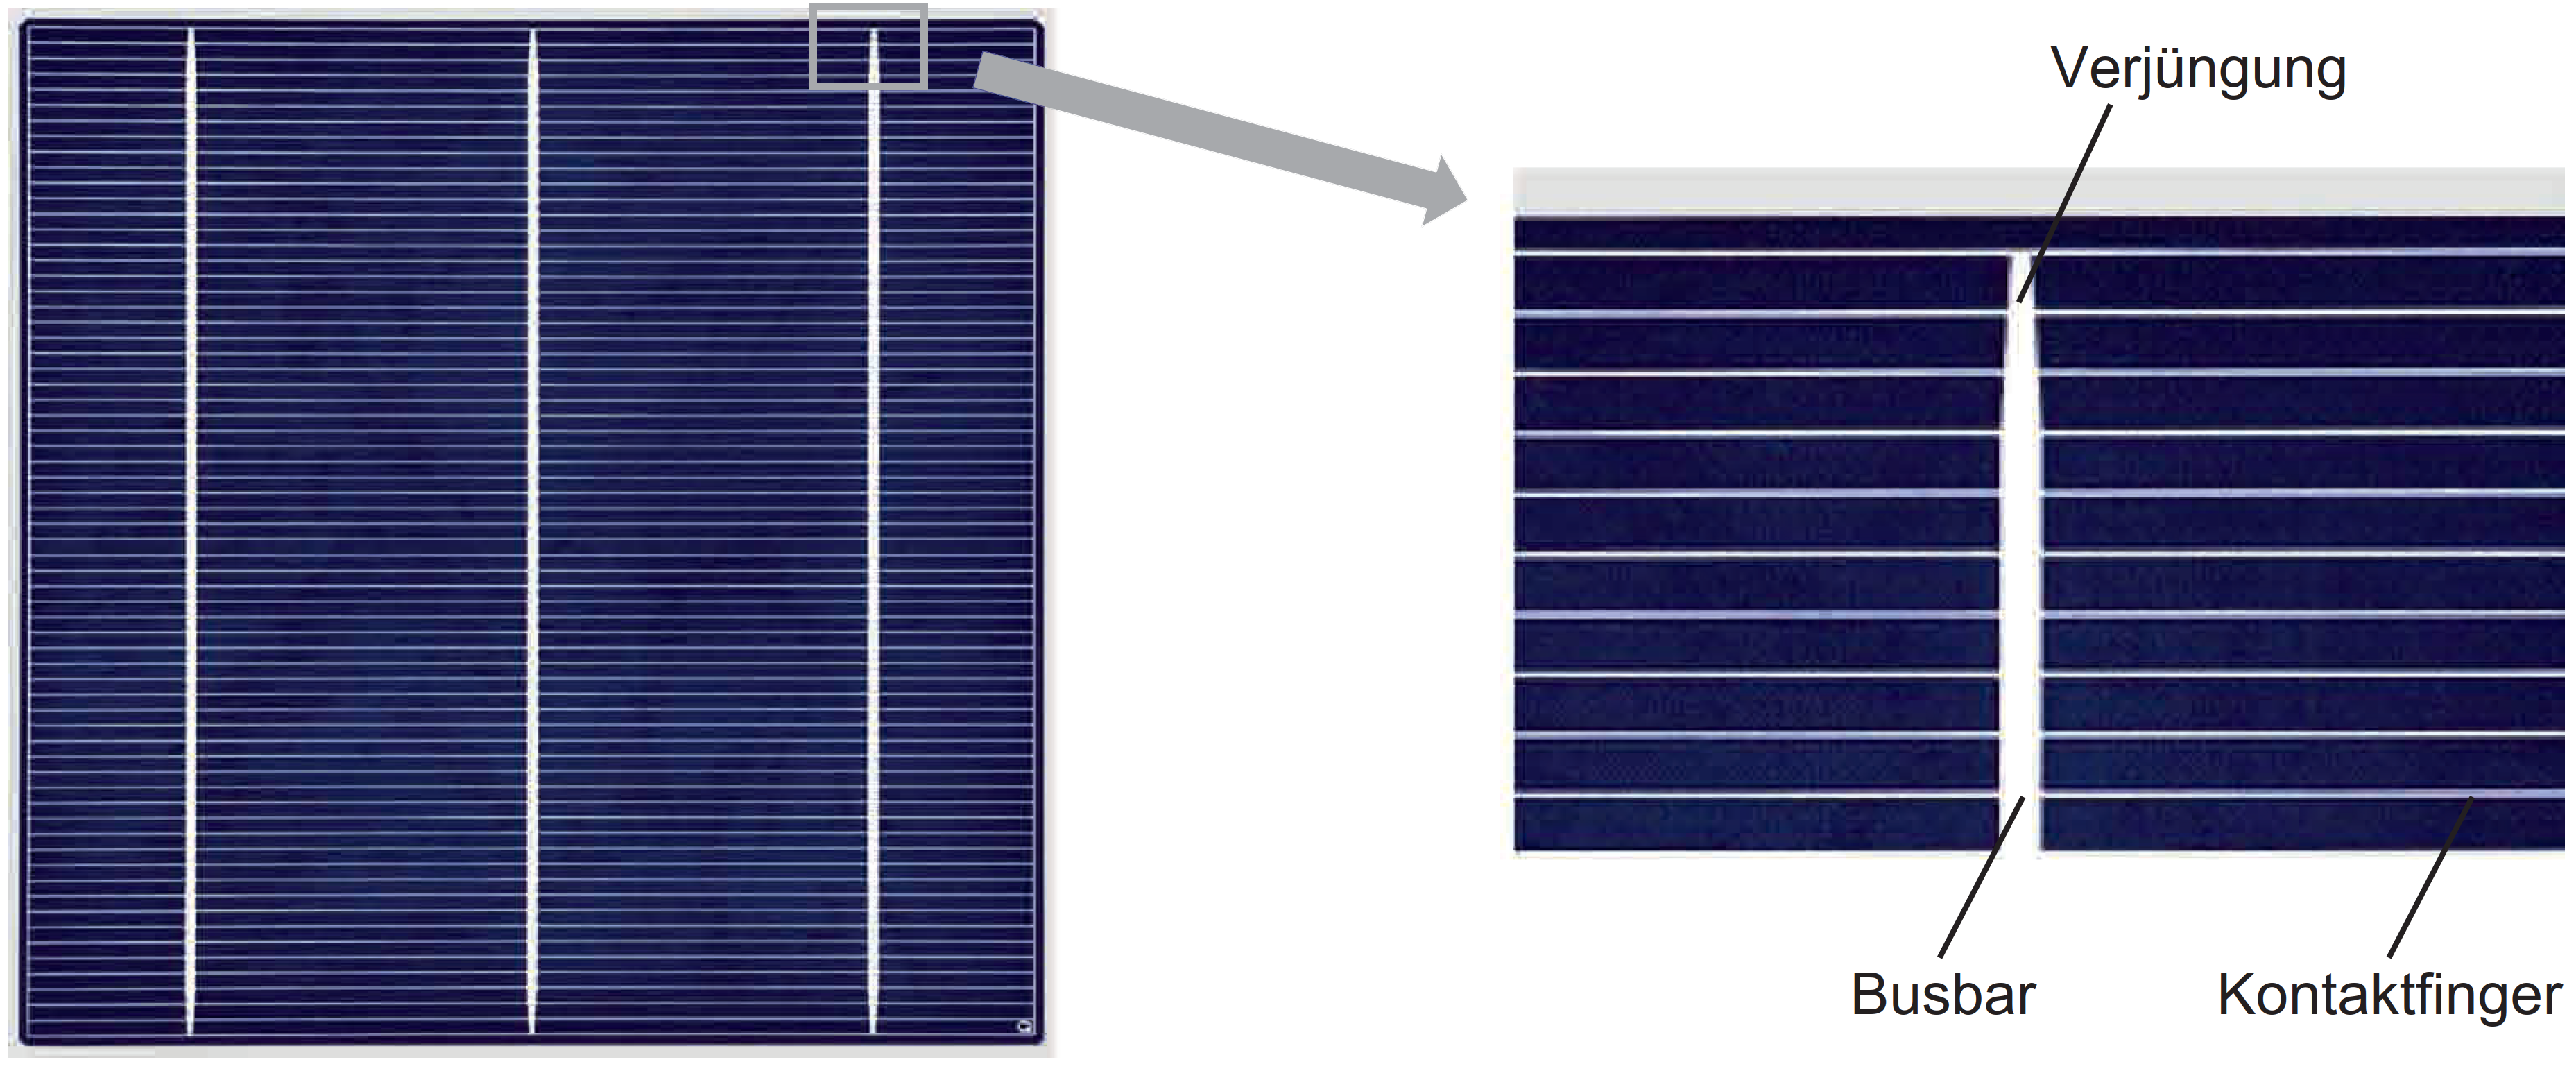
\includegraphics[width=0.95\columnwidth]{images/Frontkontakte_Solarzelle.png}
\vspace{0.2cm}
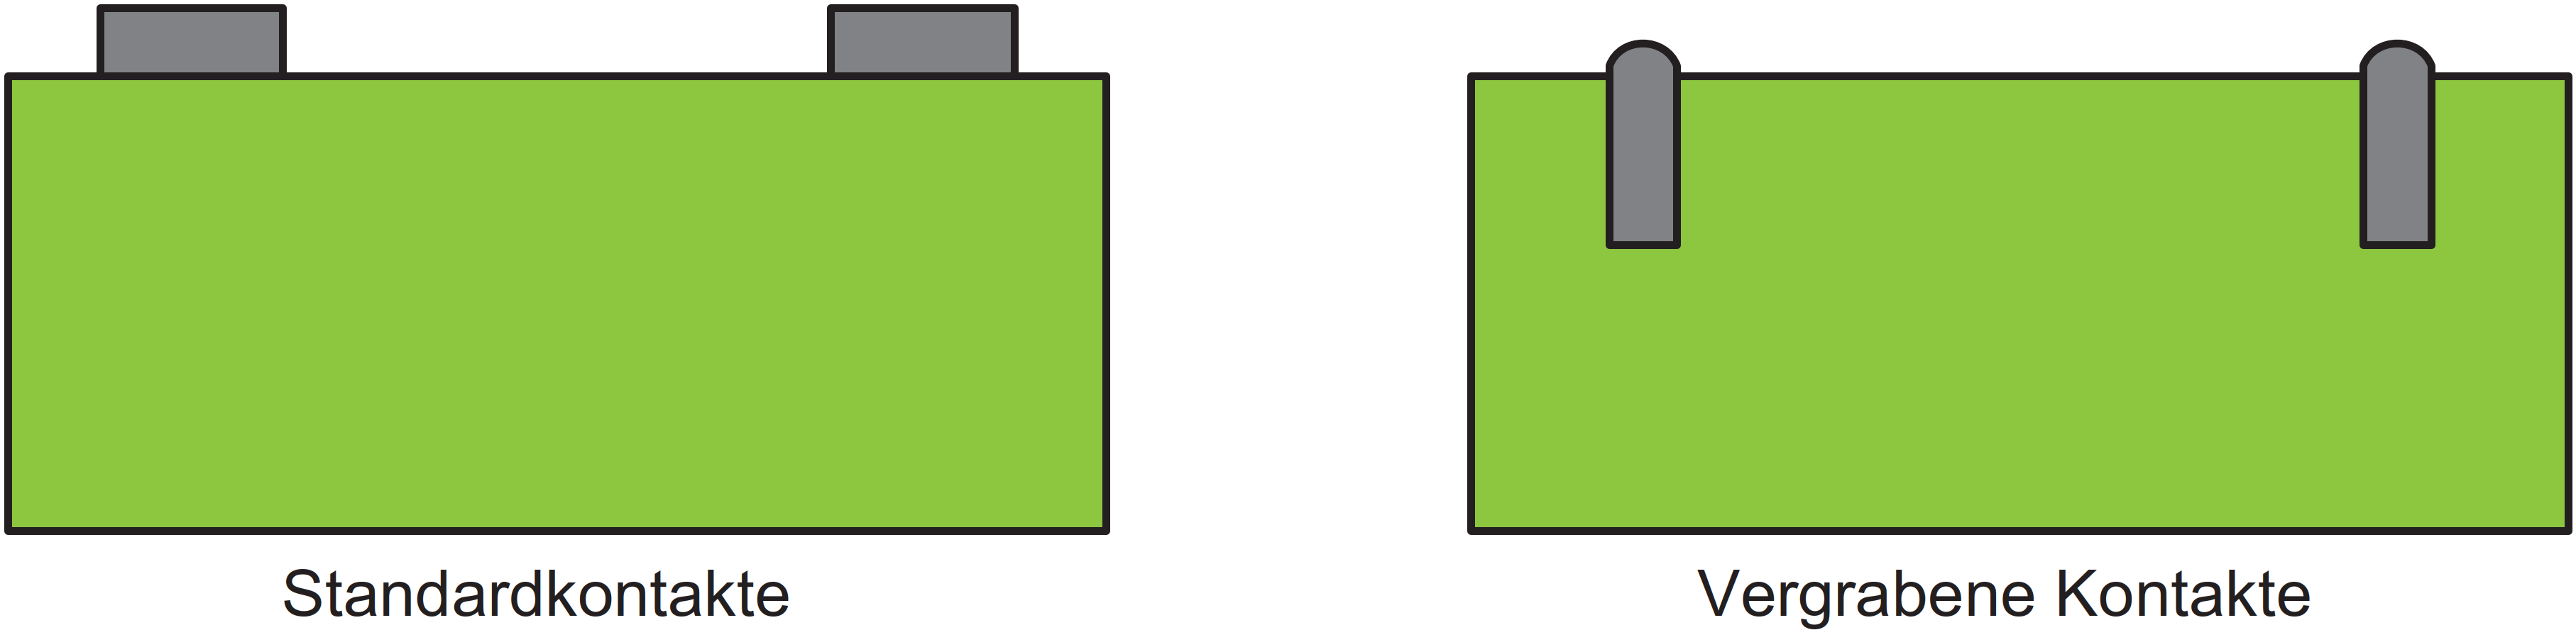
\includegraphics[width=0.95\columnwidth]{images/Standart_und_Vergrabene_Kontakte.png}
\end{center}













